% Figure M7, generated by experiments/m7_safe_screening.py.
\begin{figure}[t]
  \centering
  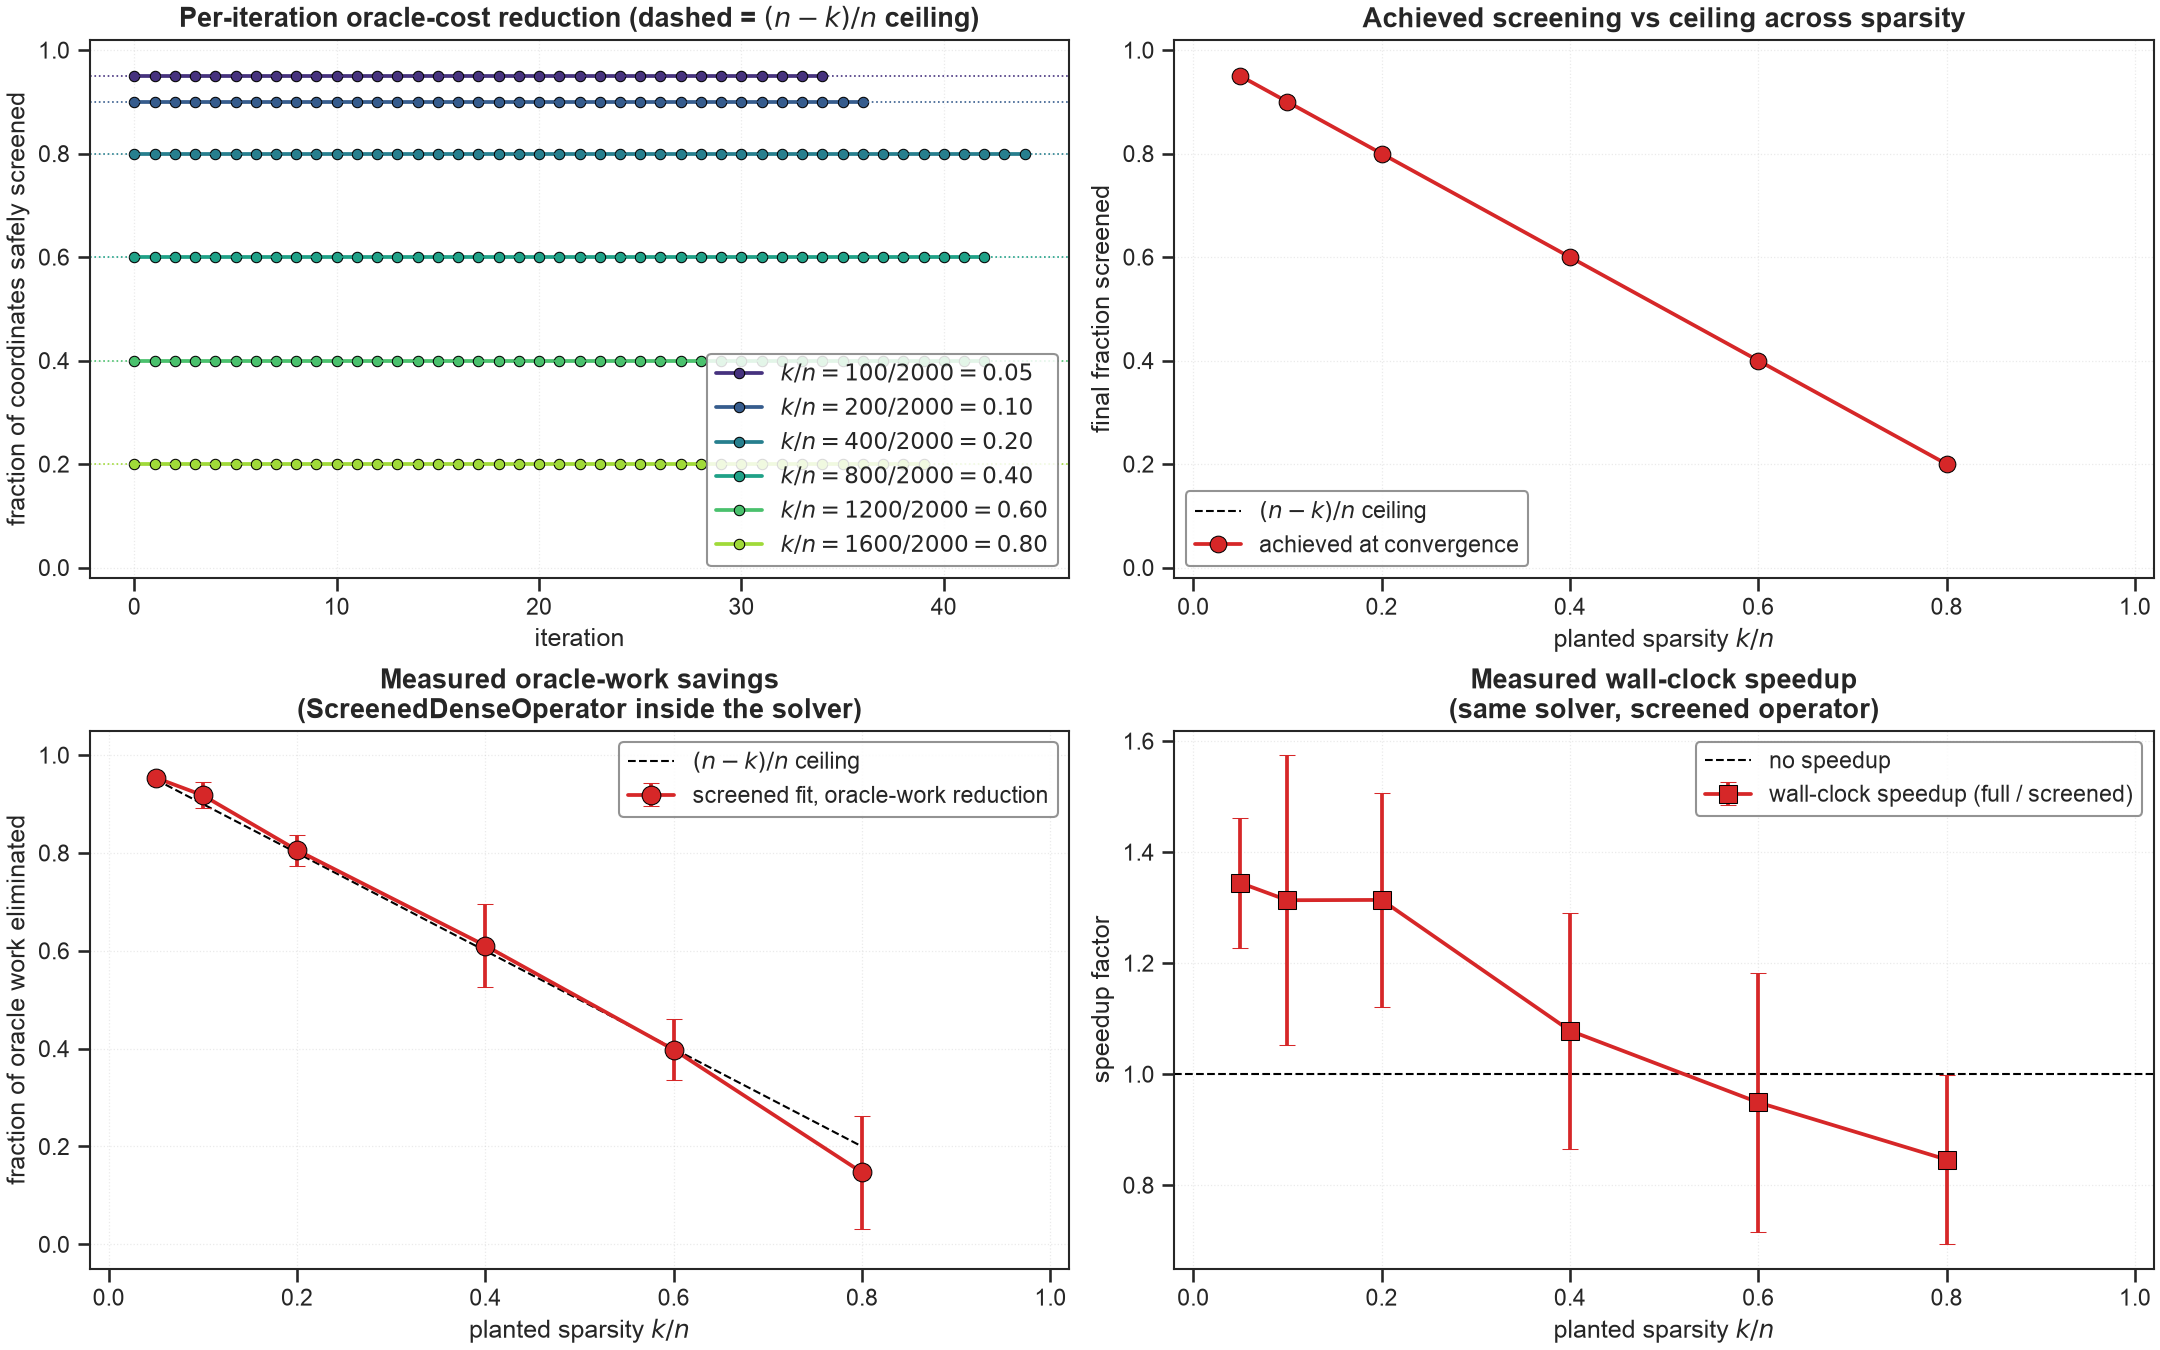
\includegraphics[width=\linewidth]{../shared/figures/generated/m7_safe_screening.png}
  \caption{\textbf{M7, A10 safe-screening payoff: advisory ceiling vs measured solver savings.} Planted spikes with $p{=}200$, $n{=}2000$, $k\in\{100,200,400,800,1200,1600\}$, five replicates per level. \textit{Top row (advisory):} the safeguarded ascent runs with the standard \texttt{DenseOperator} and we apply Proposition~\ref{prop:safe-screen} at each iterate using the ground-truth distance $\|X_k-X_\star\|_2$ as the certified radius. Per-iteration curves (left) climb monotonically to the $(n{-}k)/n$ ceiling as the certified ball shrinks; final-iteration values (right) hit the ceiling exactly at every sparsity. \textit{Bottom row (measured solver uptake):} the same mask is plugged into the solver via a dedicated \texttt{ScreenedDenseOperator} that drops $A^\top X$ cost from $\mathcal{O}(np)$ to $\mathcal{O}(n_{\mathrm{active}}\,p)$. Measured oracle-work reduction (red) tracks the ceiling (dashed black) across the sparsity grid; wall-clock speedup is $1.40\times$ at $k/n{=}0.05$ and $1.36\times$ at $k/n\in\{0.1, 0.2\}$. Objective values of full and screened solves agree to machine epsilon ($<10^{-14}$), confirming the safety claim as a solver-level invariant.}
  \label{fig:m7-safe-screening}
\end{figure}
